\documentclass[t,ignorenonframetext]{beamer}
\mode<presentation>
{
  \usetheme{Madrid}
  \usecolortheme{default}
}

\usepackage[utf8x]{inputenc}
\usepackage[francais]{babel}
\usepackage{amsmath,amsfonts,amssymb,calc}
\usepackage{listings}

\usepackage{color}
\definecolor{deepblue}{rgb}{0,0,0.5}
\definecolor{deepred}{rgb}{0.6,0,0}
\definecolor{deepgreen}{rgb}{0,0.5,0}

\newcommand{\hr}[0]{
\par{
\noindent\makebox[\linewidth]{\rule{\textwidth}{1pt}}
}
}

\newcommand\pythonstyle{\lstset{
language=Python,
otherkeywords={self},
keywordstyle=\color{deepblue},
stringstyle=\color{deepgreen},
frame=tb,
showstringspaces=false,
basicstyle=\tiny
}}
% Python environment
\lstnewenvironment{python}[1][]
{
\pythonstyle
\lstset{#1}
}
{}
% Python for external files
\newcommand\pythonexternal[2][]{{
\pythonstyle
\lstinputlisting[#1]{#2}}}

\newtheorem*{defi}{Definition}

\usefonttheme{structuresmallcapsserif}
\usepackage{enumerate,graphicx,enumerate}

\newcommand{\tc}[1]{$\backslash$\texttt{#1}}

\title{Mod\'elisation des \'ecosyst\`emes aquatiques}
\author[Yann]{Nicolas Piret \& Yann Sp\"ori}
\date{\today}
\institute[ULB]{Université Libre de Bruxelles}
\subject{}
\keywords{}

\begin{document}

% title page
\frame{
  \maketitle
%  \begin{center}
%    \small{\url{https://techfnord.de/bioinf/ulb/aqua.pdf}}
%  \end{center}
}

\frame{
  \frametitle{Diagramme conceptuel}
    \begin{figure}
      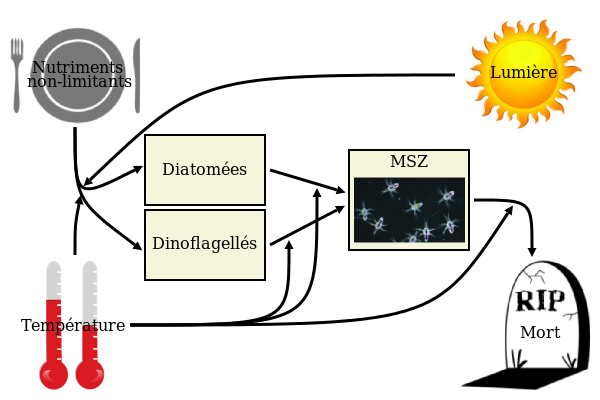
\includegraphics[width=.8\textwidth]{../partie2/diagConc.png}
    \end{figure}
}
\frame{
  \frametitle{Equations}
\begin{equation}
  {{d[DA]}\over{dt}} =
  \mu_{DA} [DA] - graz_{MSZ/DA} [MSZ]
  \label{eq:partie2DiffEq1}
\end{equation}
\begin{equation}
  {{d[DINO]}\over{dt}} =
  \mu_{DINO} [DINO] - graz_{MSZ/DINO} [MSZ]
  \label{eq:partie2DiffEq2}
\end{equation}
\begin{equation}
  {{d[MSZ]}\over{dt}} =
  \left (
    (1- eges_{MSZ}) graz_{MSZ} Y_{MSZ} - mm_{MSZ}
  \right ) [MSZ]
  \label{eq:partie2DiffEq3}
\end{equation}
}
\frame{
  \frametitle{Grazing sélectif}
\begin{equation}
  [PHYTO] = [DA] + [DINO]
  \label{eq:partie2nonSelEq1}
\end{equation}
\begin{equation}
  graz_{MSZ} = g_{MSZ} max(T) {{[PHYTO]^2}\over{kg_{MSZ}^2 + [PHYTO]^2}}
  \label{eq:partie2nonSelEq2}
\end{equation}
\begin{equation}
  graz_{MSZ/DA} = graz_{MSZ} {{[DA]}\over{[PHYTO]}}
  \label{eq:partie2nonSelEq2}
\end{equation}
\begin{equation}
  graz_{MSZ/DINO} = graz_{MSZ} {{[DINO]}\over{[PHYTO]}}
  \label{eq:partie2nonSelEq3}
\end{equation}
}
\frame{
  \frametitle{Grazing non-sélectif}
\begin{equation}
  graz_{MSZ/DA} = g_{MSZ} max(T) {{\left ( {{[DA]}\over{kg_{MSZ/DA}}}\right )^2}\over
{1 + \left ( {{[DA]}\over{kg_{MSZ/DA}}} \right )^2 + \left ( {{[DINO]}\over{kg_{MSZ/DINO}}} \right )^2}}
  \label{eq:partie2selEq1}
\end{equation}
\begin{equation}
  graz_{MSZ/DINO} = g_{MSZ} max(T) {{\left ( {{[DINO]}\over{kg_{MSZ/DINO}}}\right )^2}\over
{1 + \left ( {{[DA]}\over{kg_{MSZ/DA}}} \right )^2 + \left ( {{[DINO]}\over{kg_{MSZ/DINO}}} \right )^2}}
  \label{eq:partie2selEq2}
\end{equation}
\begin{equation}
  graz_{MSZ} = g_{MSZ/DA} + g_{MSZ/DINO}
  \label{eq:partie2selEq3}
\end{equation}
}
\frame{
  \frametitle{Simulations de référence}
    \begin{figure}
      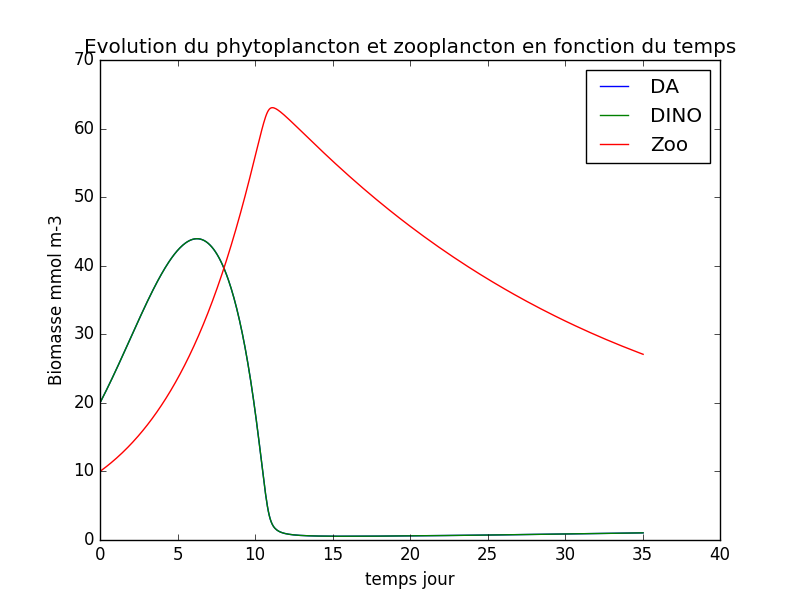
\includegraphics[width=0.5\textwidth]{../partie2/1Nonselec.png}\hfill
      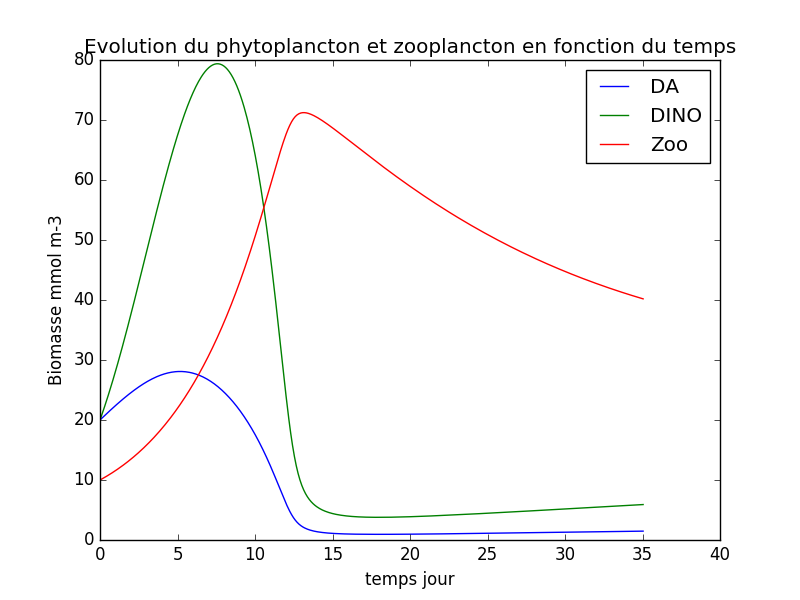
\includegraphics[width=0.5\textwidth]{../partie2/1Selec.png}\hfill
      \caption{Les simulations de référence. Le graphique à gauche montre
le cas d'une fonction de grazing non séléctive et le graphique à droite montre le cas
d'une fonction de grazing séléctive.}
    \end{figure}
}

\frame{
  \frametitle{Test 1 - grazing non-sélectif}
    \begin{figure}
      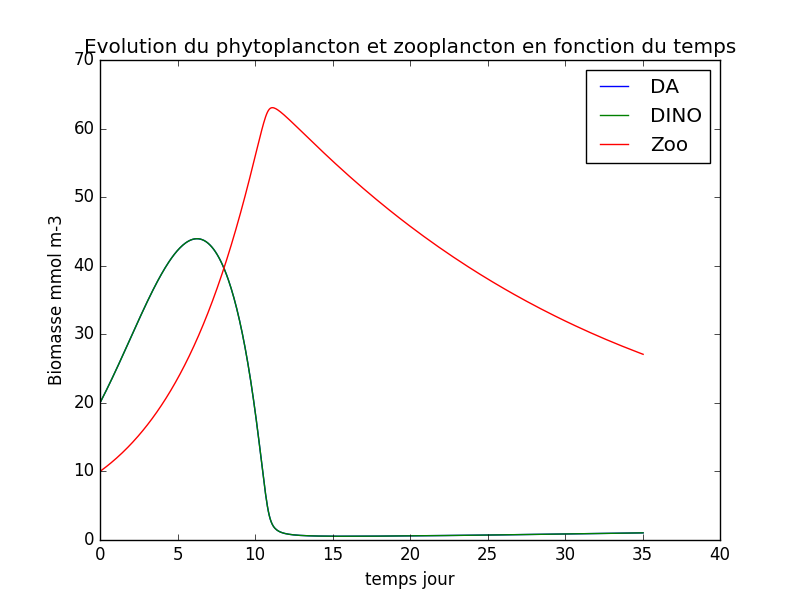
\includegraphics[width=0.5\textwidth]{../partie2/1Nonselec.png}\hfill
      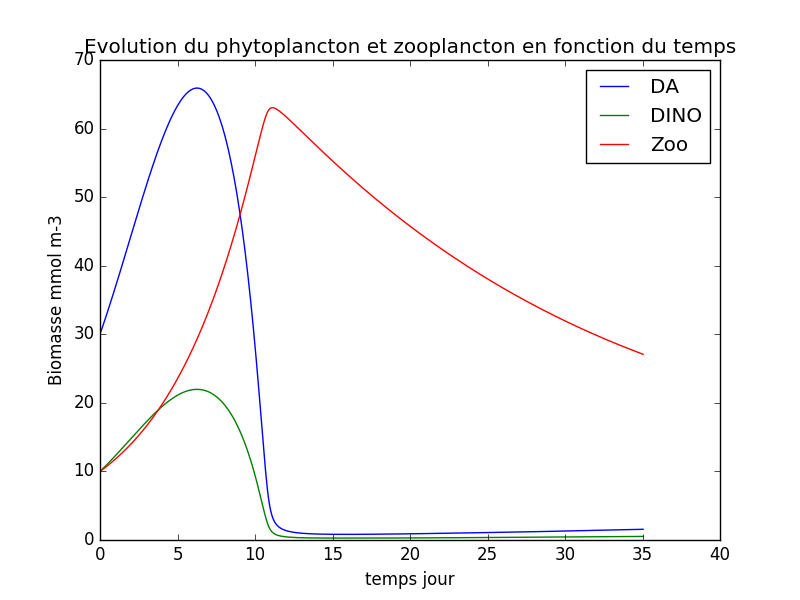
\includegraphics[width=0.5\textwidth]{../partie2/test1nonsel.png}\hfill
      \caption{La simulation de référence (gauche) par rapport au premier test de sensibilité (droite).
Dans le premier test, on a augmenté la valeur initiale du $DA$ de 20 à 30 $^{mmol~C}/_{m^{-3}}$ et on a
diminué la valeur initiale du $DINO$ de 20 à 10 $^{mmol~C}/_{m^{-3}}$.
}
    \end{figure}
}
\frame{
  \frametitle{Test 1 - grazing séléctif}
    \begin{figure}
      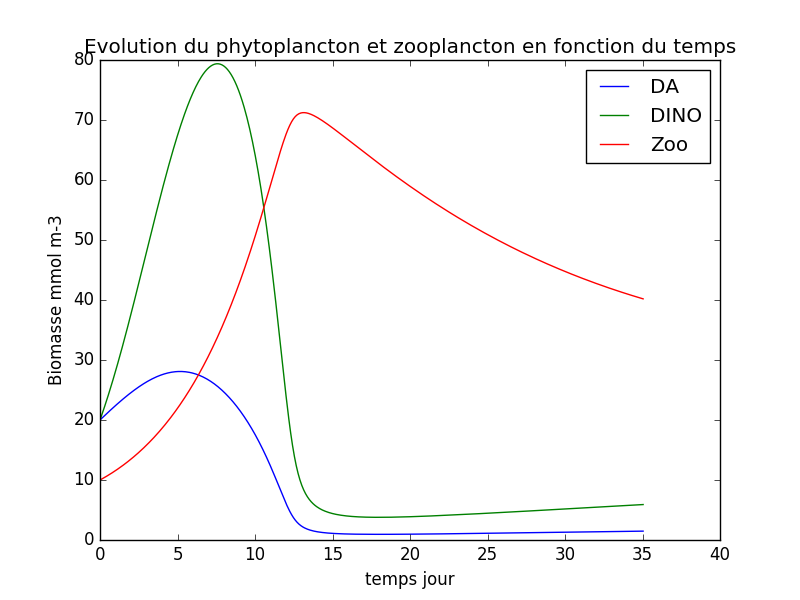
\includegraphics[width=0.5\textwidth]{../partie2/1Selec.png}\hfill
      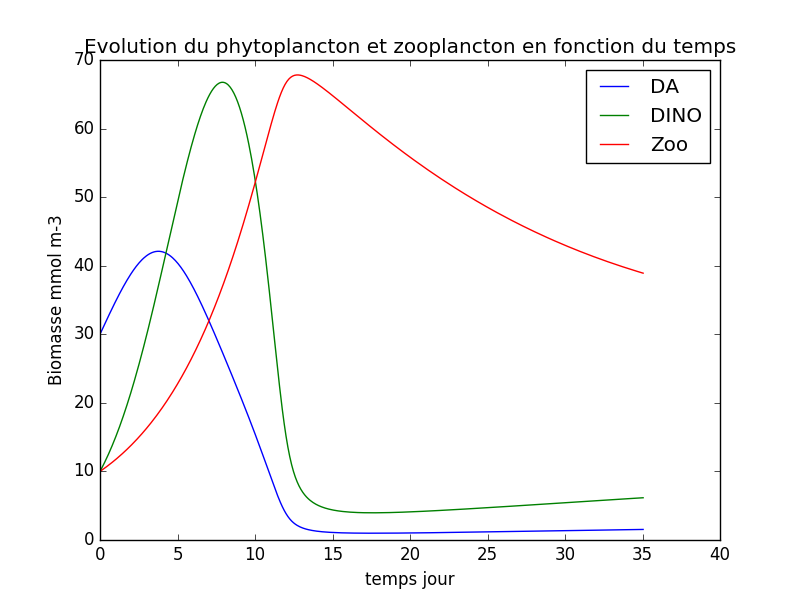
\includegraphics[width=0.5\textwidth]{../partie2/test1sel.png}\hfill
      \caption{La simulation de référence (gauche) par rapport au premier test de sensibilité (droite).
Dans le premier test, on a augmenté la valeur initiale du $DA$ de 20 à 30 $^{mmol~C}/_{m^{-3}}$ et on a
diminué la valeur initiale du $DINO$ de 20 à 10 $^{mmol~C}/_{m^{-3}}$.
      }
    \end{figure}
}

\frame{
  \frametitle{Test 2 - grazing non-sélectif}
    \begin{figure}
      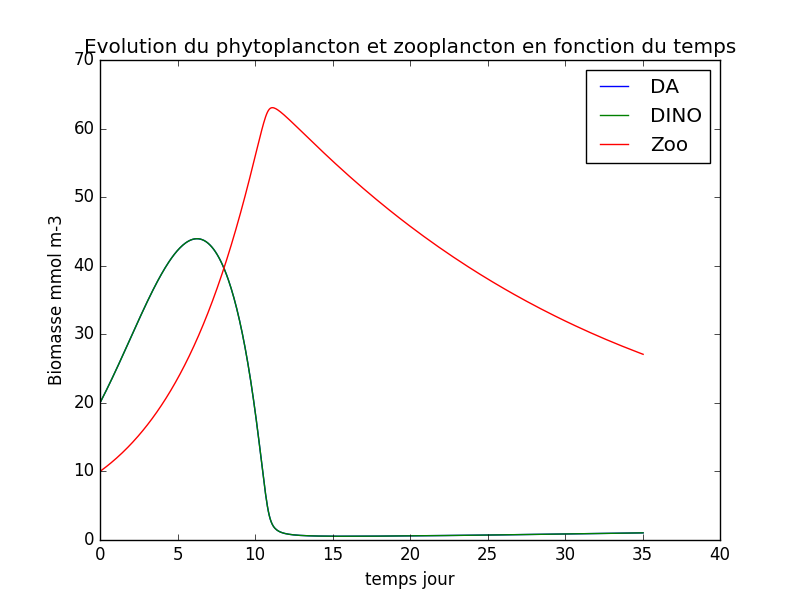
\includegraphics[width=0.5\textwidth]{../partie2/1Nonselec.png}\hfill
      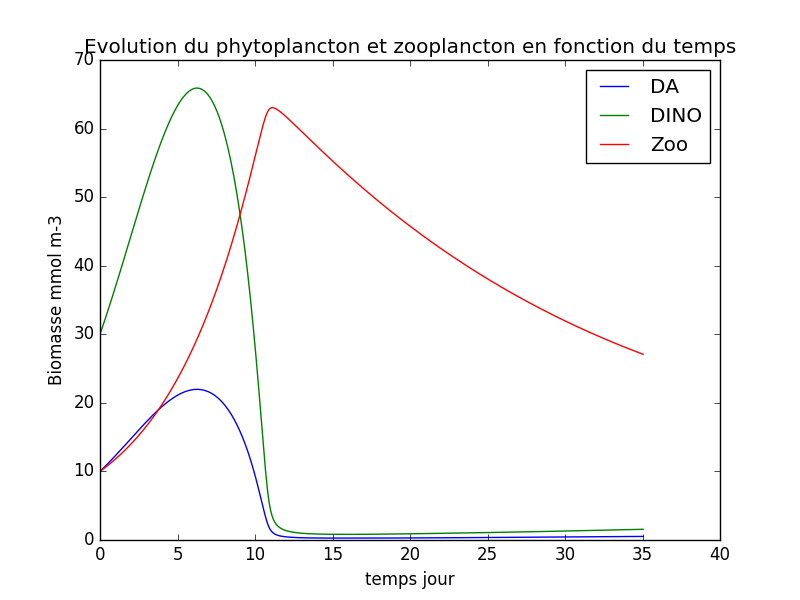
\includegraphics[width=0.5\textwidth]{../partie2/test2nonsel.png}\hfill
      \caption{La simulation de référence (gauche) par rapport au deuxième test de sensibilité (droite).
Dans le deuxième test, on a augmenté la valeur initiale du $DINO$ de 20 à 30 $^{mmol~C}/_{m^{-3}}$ et on a
diminué la valeur initiale du $DA$ de 20 à 10 $^{mmol~C}/_{m^{-3}}$.
}
    \end{figure}
}
\frame{
  \frametitle{Test 2 - grazing sélectif}
    \begin{figure}
      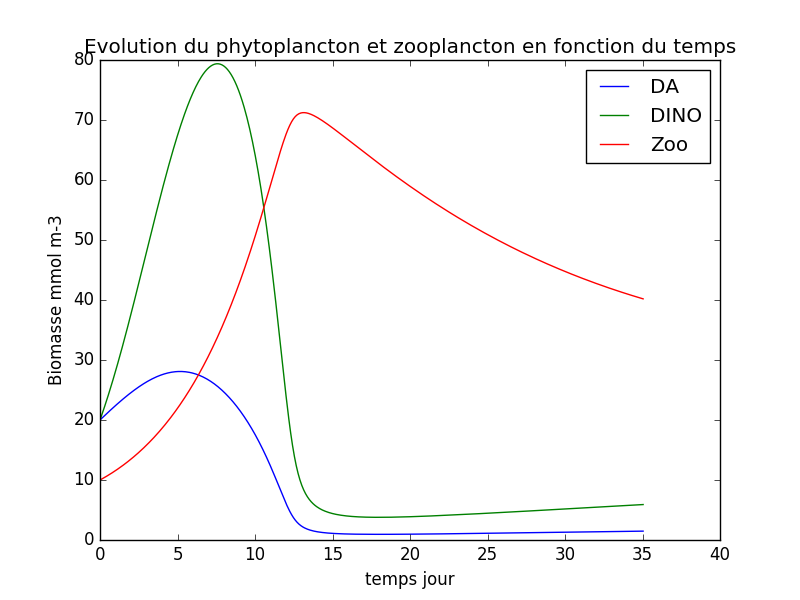
\includegraphics[width=0.5\textwidth]{../partie2/1Selec.png}\hfill
      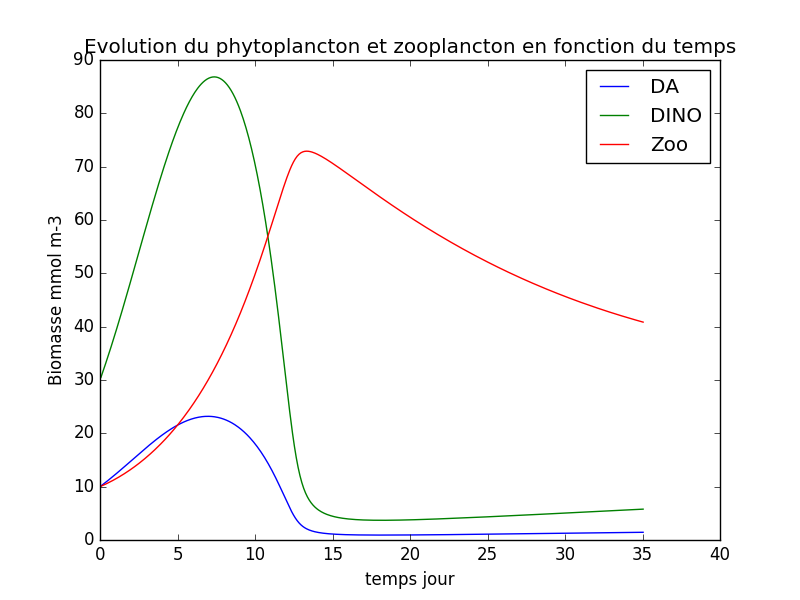
\includegraphics[width=0.5\textwidth]{../partie2/test2sel.png}\hfill
      \caption{La simulation de référence (gauche) par rapport au deuxième test de sensibilité (droite).
Dans le deuxième test, on a augmenté la valeur initiale du $DINO$ de 20 à 30 $^{mmol~C}/_{m^{-3}}$ et on a
diminué la valeur initiale du $DA$ de 20 à 10 $^{mmol~C}/_{m^{-3}}$.
}
    \end{figure}
}

\frame{
  \frametitle{Test 3 - grazing non-sélectif}
    \begin{figure}
      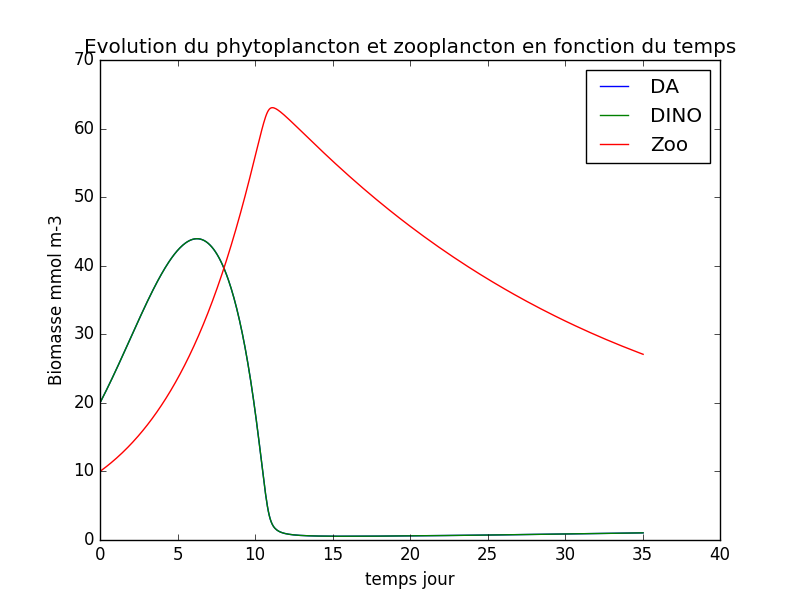
\includegraphics[width=0.5\textwidth]{../partie2/1Nonselec.png}\hfill
      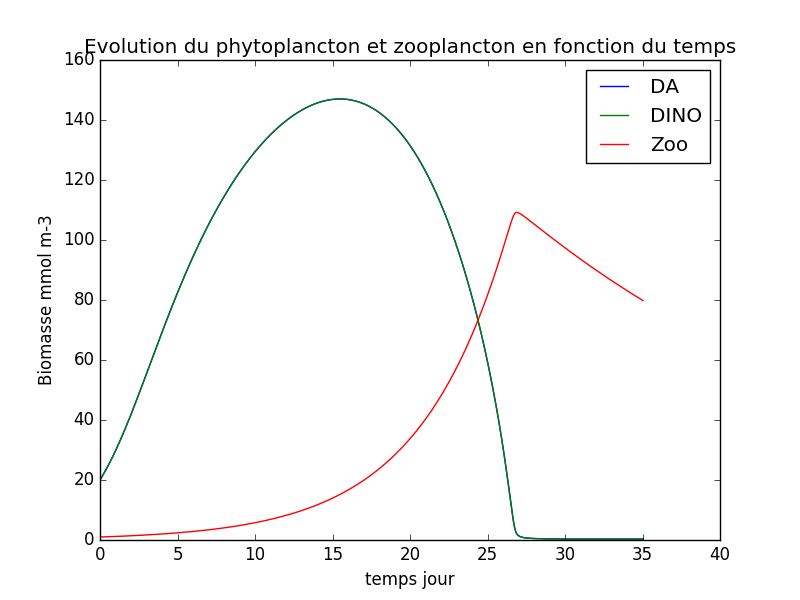
\includegraphics[width=0.5\textwidth]{../partie2/test3nonsel.png}\hfill
      \caption{La simulation de référence (gauche) par rapport au troisième test de sensibilité (droite).
Dans le troisième test, on a diminué la valeur initiale du $MSZ$ de 10 à 1 $^{mmol~C}/_{m^{-3}}$.
}
    \end{figure}
}
\frame{
  \frametitle{Test 3 - grazing sélectif}
    \begin{figure}
      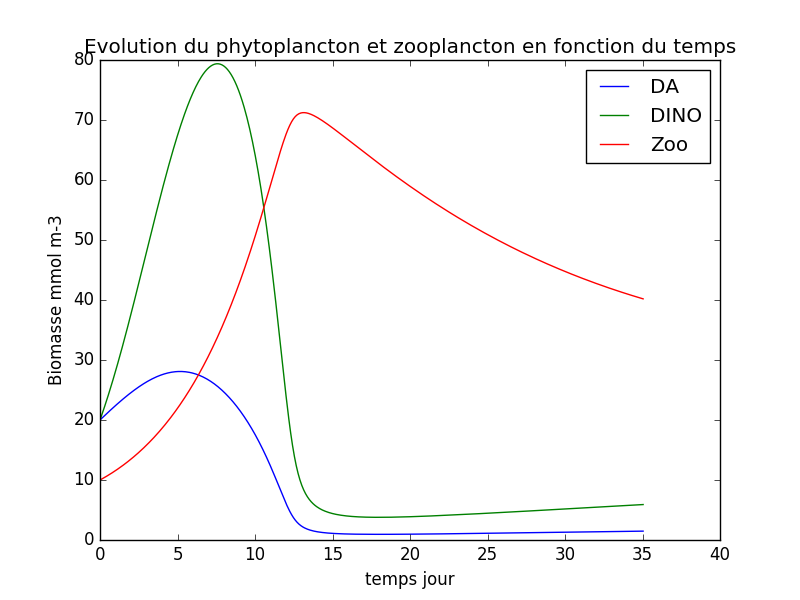
\includegraphics[width=0.5\textwidth]{../partie2/1Selec.png}\hfill
      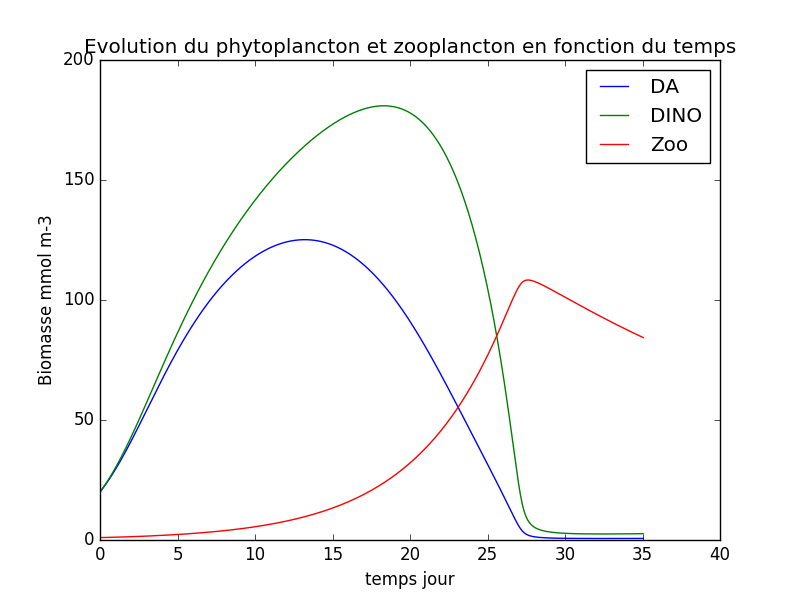
\includegraphics[width=0.5\textwidth]{../partie2/test3sel.png}\hfill
      \caption{La simulation de référence (gauche) par rapport au troisième test de sensibilité (droite).
Dans le troisième test, on a diminué la valeur initiale du $MSZ$ de 10 à 1 $^{mmol~C}/_{m^{-3}}$.
}
    \end{figure}
}

\frame{
  \frametitle{Test 4 - grazing non-sélectif}
    \begin{figure}
      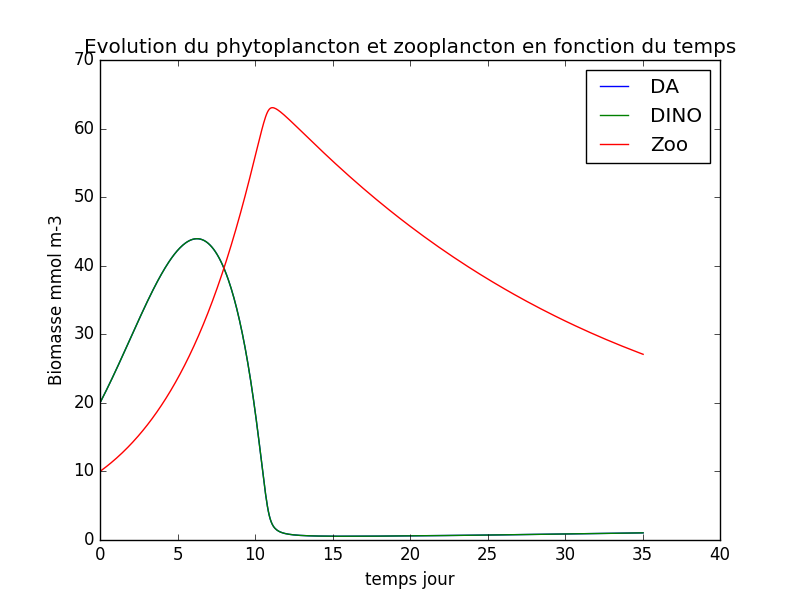
\includegraphics[width=0.5\textwidth]{../partie2/1Nonselec.png}\hfill
      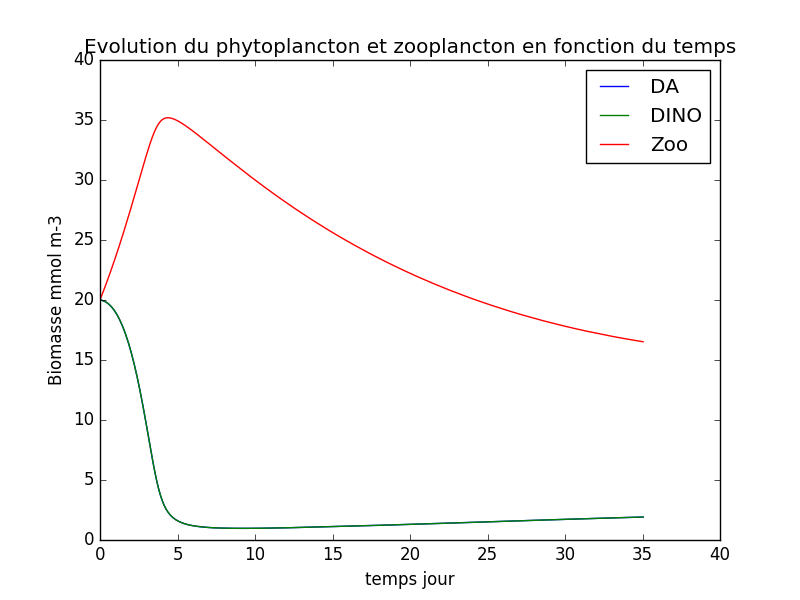
\includegraphics[width=0.5\textwidth]{../partie2/test4nonsel.png}\hfill
      \caption{La simulation de référence (gauche) par rapport au quatrième test de sensibilité (droite).
Dans le quatrième test, on a augmenté la valeur initiale du $MSZ$ de 10 à 20 $^{mmol~C}/_{m^{-3}}$.
}
    \end{figure}
}
\frame{
  \frametitle{Test 4 - grazing sélectif}
    \begin{figure}
      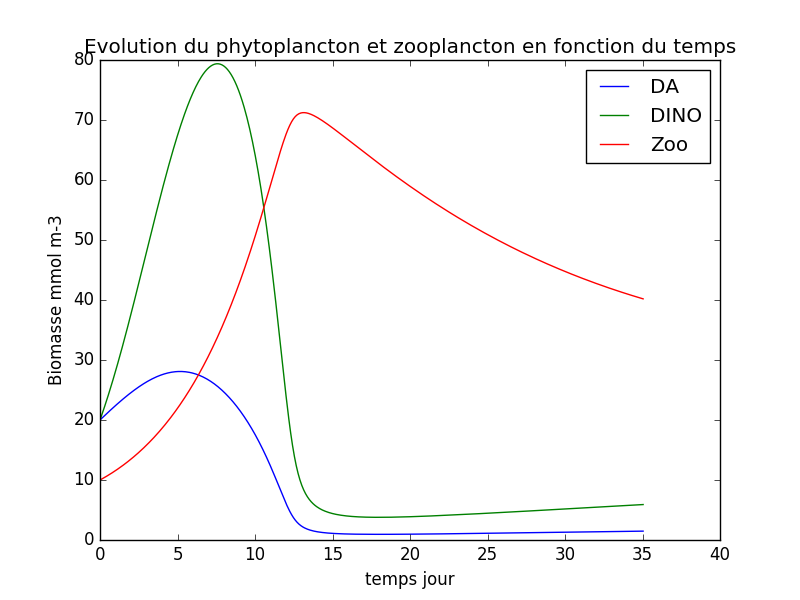
\includegraphics[width=0.5\textwidth]{../partie2/1Selec.png}\hfill
      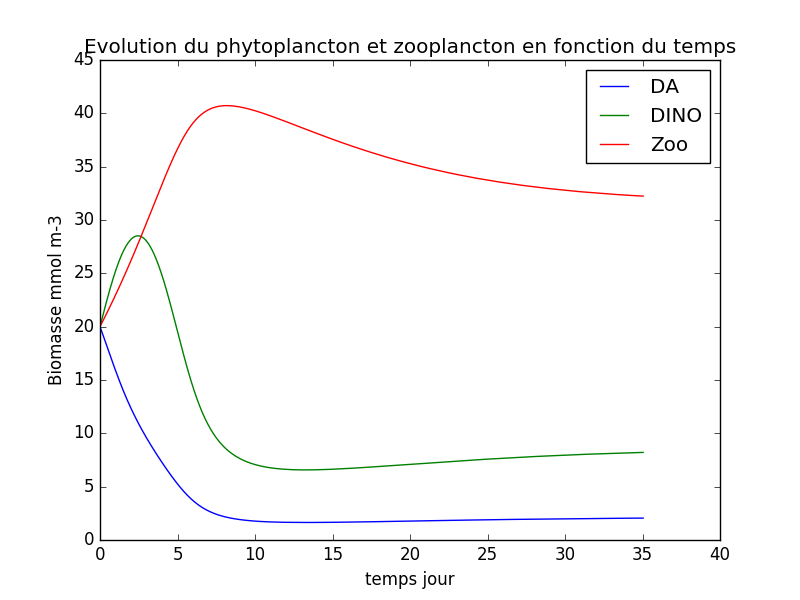
\includegraphics[width=0.5\textwidth]{../partie2/test4sel.png}\hfill
      \caption{La simulation de référence (gauche) par rapport au quatrième test de sensibilité (droite).
Dans le quatrième test, on a augmenté la valeur initiale du $MSZ$ de 10 à 20 $^{mmol~C}/_{m^{-3}}$.
}
    \end{figure}
}
\frame{
  \frametitle{Questions?}
  \vfill
  \begin{center}
   \LARGE{??? QUESTIONS ???}
  \end{center}
  \vfill
}

\end{document}
